Si riporta nel seguito un breve aggiornamento sulle novità principali avvenute nei mesi che vanno dalla stesura del presente documento (Dicembre 2017) alla sua presentazione (Aprile 2018).

\paragraph{Il crollo delle criptovalute} ~ \\
    Le dichiarazioni del governo sudcoreano prospettanti un possibile blocco delle criptovalute, avvenute a metà gennaio, hanno inaugurato un periodo difficoltoso per il mercato delle monete basate su blockchain. Prendendo come riferimento Bitcoin, che si mantiene al primo posto per quanto riguarda il valore di mercato e pertanto riflette piuttosto bene l'andamento generale, dopo aver raggiunto il picco di circa 19'500 dollari a metà dicembre ha visto il suo valore crollare a poco meno di 7'000 dollari, con giornate particolarmente critiche che hanno registrato svalutazioni di oltre il 10\% nell'arco di 24 ore.

    \begin{figure}[ht]
        \centering
        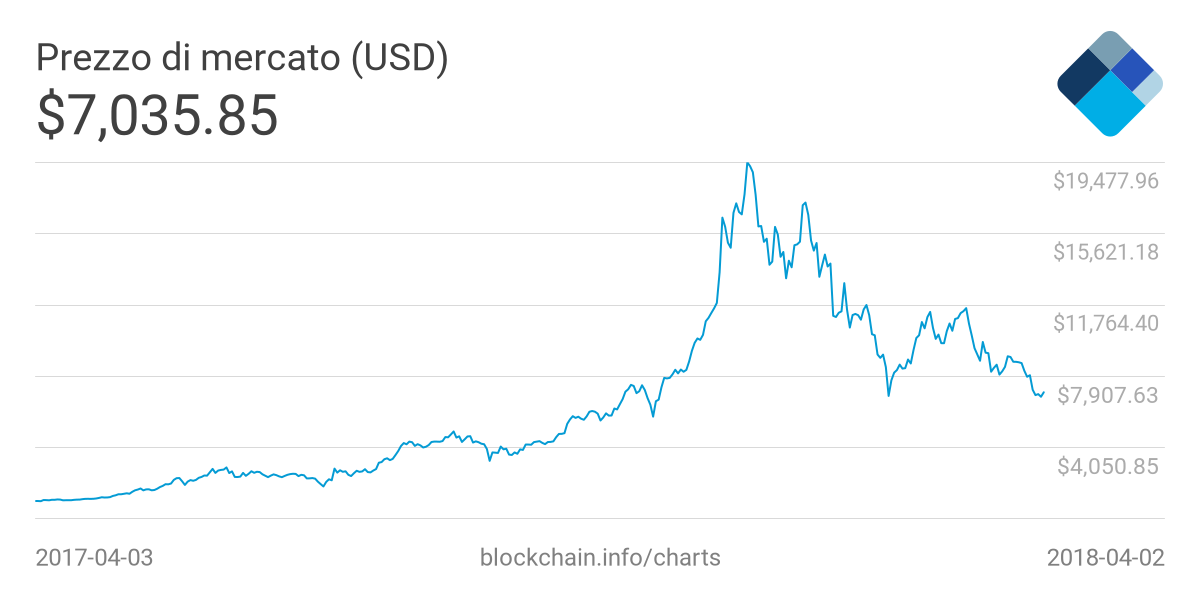
\includegraphics[width=\textwidth]{bitcoin-price-update.png}
        \caption[Valore di Bitcoin nell'ultimo anno]{Valore di Bitcoin nell'ultimo anno.}
        \label{fig:bitcoin-price-update}
    \end{figure}

    Conseguenza diretta di questa contrazione è stata la rivalutazione da parte dell'opinione pubblica riguardo a Bitcoin e blockchain in generale, e l'abbandono dei toni sensazionalisti adottati negli ultimi mesi del 2017. Il tutto rispecchia l'analisi di Gartner riportata in introduzione (\hyperref[sec:introduzione]{Cap. \ref*{sec:introduzione}}), e rimette nella giusta prospettiva un fenomeno tanto impattante quanto bisognoso di cautela nella propria gestione.

\paragraph{Primi test di carico per Ethereum} ~ \\
    Anche Ethereum si è trovata interessata da un considerevole aumento di carico, con il picco massimo nel mese di gennaio, dovuto alla diffusione dei \emph{Crypto Kitties}. Si tratta di animaletti digitali, simili ai più datati Tamagochi, che vivono e si riproducono nella blockchain di Ethereum alimentando un correlato mercato di collezionisti. Il traffico da loro generato è arrivato a rappresentare oltre il 20\% del traffico totale di Ethereum, il quale si è mostrato capace di affrontare l'impennata di transazioni adeguatamente seppure con una risposta iniziale piuttosto lenta che ha fatto temere per il congestionamento del sistema.

    \begin{figure}[ht]
        \centering
        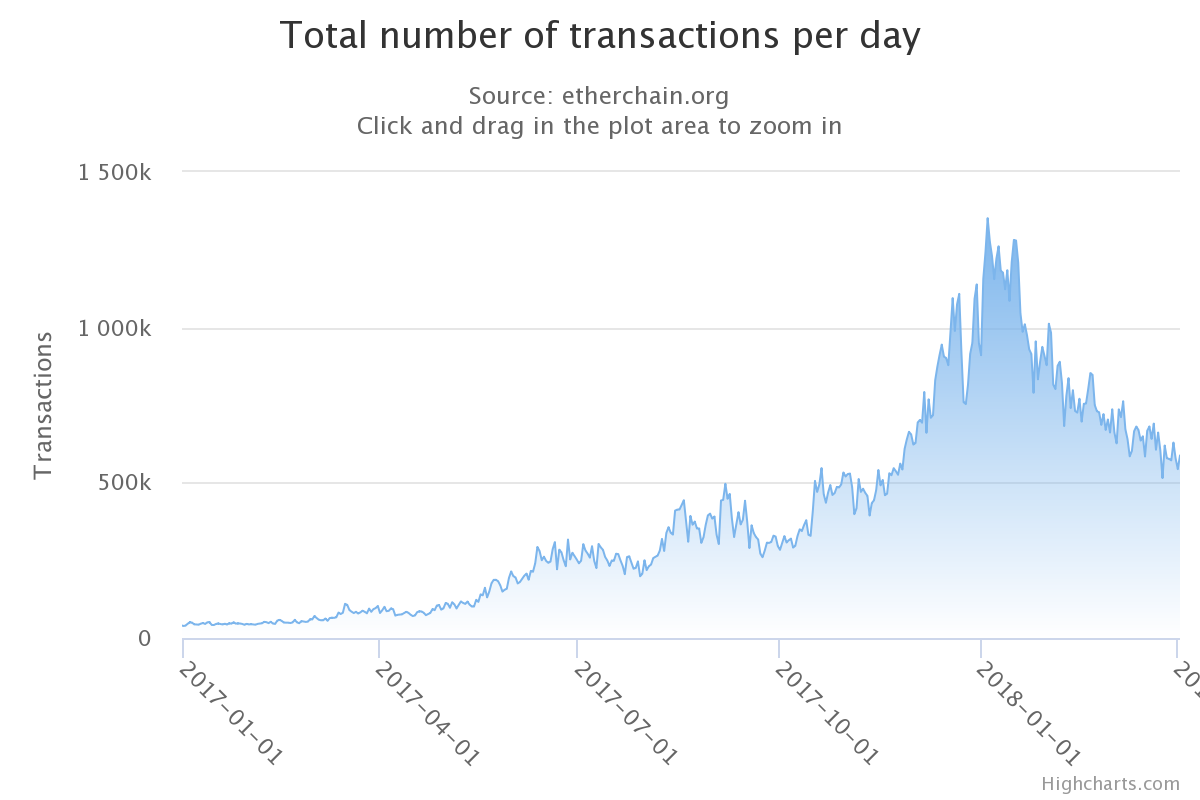
\includegraphics[width=\textwidth]{ethereum-load.png}
        \caption[Numero di transazioni giornaliere su Ethereum]{Numero di transazioni giornaliere su Ethereum.}
        \label{fig:ethereum-load}
    \end{figure}

\paragraph{La situazione dell'ecosistema} ~ \\
    L'intero ecosistema che ruota attorno alla tecnologia blockchain è stato condizionato dalla disillusione portata dal crollo delle criptovalute. Molti progetti si sono arenati e, in generale, ci si sta rendendo conto delle difficoltà di sviluppo e mantenimento di tali sistemi \cite{blockchain_delusion}.

    In compenso, alcuni progetti hanno raggiunto la piena maturità, come Hyperledger Sawtooth (citato nella \hyperref[sec:non-crypto]{Sez. \ref*{sec:non-crypto}}) che ha raggiunto la versione 1.0.1. Anche nell'ambito dei sistemi di identità digitale si registrano passi avanti nel campo della standardizzazione e dello sviluppo attraverso i lavori congiunti di \emph{W3C}, la community \emph{Rebooting The Web Of Trust} \cite{rebooting_web_of_trust} e Hyperledger Indy.

    Da segnalare anche lo sviluppo di IOTA, DLT basato su una struttura dati alternativa a blockchain ma basata su concetti simili. Si tratta di un DAG, un grafo orientato aciclico, che può essere immaginato come un reticolo formato da più blockchain intrecciate - ciascuna transazione deve approvarne due precedenti - e questa struttura dati sembra molto più veloce di una blockchain ``tradizionale'' pur mantenendone l'affidabilità. Maggiori approfondimenti richiedono spiegazioni più dettagliate e corpose, che si possono trovare all'indirizzo \url{https://iota.org/}.